\documentclass[letterpaper,pdftex]{article}

\setlength{\textwidth}{168mm}
\setlength{\textheight}{210mm}
\setlength{\oddsidemargin}{0cm}
\setlength{\topmargin}{0cm}
\setlength{\headheight}{48pt}
\addtolength{\textheight}{-25pt}
\voffset -0.5in

\usepackage{natbib}
\usepackage[utf8]{inputenc}
\usepackage[spanish]{babel}
\usepackage{xcolor,graphicx}
\usepackage{fancyhdr}
\usepackage{multirow}
\usepackage{siunitx}
\usepackage{hyperref}
\hypersetup{
    colorlinks,
    citecolor=blue,
    filecolor=black,
    linkcolor=blue,
    urlcolor=black
}
\usepackage{epstopdf}
%To code editing
\usepackage{listings}
\usepackage{xcolor}
\definecolor{codegreen}{rgb}{0,0.6,0}
\definecolor{codegray}{rgb}{0.5,0.5,0.5}
\definecolor{codepurple}{rgb}{0.58,0,0.82}
\definecolor{backcolour}{rgb}{0.95,0.95,0.92}

\lstdefinestyle{mystyle}{
    backgroundcolor=\color{backcolour},   
    commentstyle=\color{codegreen},
    keywordstyle=\color{magenta},
    numberstyle=\tiny\color{codegray},
    stringstyle=\color{codepurple},
    basicstyle=\ttfamily\footnotesize,
    breakatwhitespace=false,         
    breaklines=true,                 
    captionpos=b,                    
    keepspaces=true,                 
    numbers=left,                    
    numbersep=5pt,                  
    showspaces=false,                
    showstringspaces=false,
    showtabs=false,                  
    tabsize=2
}

\lstset{style=mystyle}
% --------------

\usepackage[autolinebreaks,useliterate]{mcode}
\pagestyle{fancy}
\renewcommand{\headrule}{\color{gray}
\hrule width\headwidth height\headrulewidth \vskip-\headrulewidth}
\renewcommand{\footrule}{{\color{gray}
\vskip-\footruleskip\vskip-\footrulewidth
\hrule width\headwidth height\footrulewidth\vskip\footruleskip}}
\renewcommand{\headrulewidth}{1.5pt}
\renewcommand{\footrulewidth}{1.5pt}

\usepackage{caption}
\usepackage{subcaption}

\spanishdecimal{.}

\begin{document}
\fancyhead{}
\fancyfoot{}
\fancyhead[L]{
\begin{minipage}{3.5cm}
\begin{center}
	
\includegraphics[width=0.95\textwidth]{logousb.png}
\end{center}
\end{minipage}
\begin{minipage}{12cm}
\begin{flushleft}
\small \textsc{Universidad de San Buenaventura}\\
\small \textsc{Faculty of Engineeering}\\
\small \textsc{School of Mechatronics Engineering\\}
\end{flushleft}
\end{minipage}
}
\fancyhead[R]{
\begin{minipage}{3.0cm}
\begin{flushright}
\small \textsc{Foundations of Robotics\\ Laboratory 2}\\
\small \textsc{2021-II}
\end{flushright}
\end{minipage}
}
\fancyfoot[R]{\large \textbf{\thepage}}

\begin{minipage}{0.3\textwidth}
\begin{flushleft}
\textbf{Author:}\\
\textit{Nikolay Prieto Ph.D(c)}\\
\end{flushleft}
\end{minipage}
\begin{minipage}{0.7cm}
\textcolor{gray}{\rule{0.3cm}{2.5cm}}
\end{minipage}
\begin{minipage}{0.64\textwidth}
\Large{\textbf{Computational Laboratory \\ ROS (Part I-A)}}
\end{minipage}\\

\noindent
\textcolor{gray}{\rule{\textwidth}{0.5pt}}\\
\renewcommand{\tablename}{Tabla}
\renewcommand{\arraystretch}{1.2}
\renewcommand\contentsname{Contents}
\tableofcontents

\noindent
\textcolor{gray}{\rule{\textwidth}{0.5pt}}\\

\section{Objectives}
\begin{itemize}
\item To get a practical knowledge of the basic concepts related to how ROS (\textit{Robot Operating System}) works.
\item To show robot models in RViz, a ROS visualizer, and interact with the models through the default interface and code.
\item To send joint positions from ROS to a simulated robot in the dynamic Gazebo simulator.
\end{itemize}

\section{Equipment and Materials}
\begin{itemize}
\item Ros version: Noetic
\item OS: linux Ubuntu 18.04 or above.
\item Gazebo v9.0 or above.
\end{itemize}

\section{General Considerations}
\subsection{About the Report}
\begin{itemize}
\item Provide answers to the questions of this guide in a separate document using any text
editor such as word, latex, etc.
\item When needed, or when explicitly required, insert the source code and some visible
screenshots of the results.
\item The lab report must be submitted via Teams (See assignment) in PDF format.
\end{itemize} 

\subsection{About the laboratory}
\begin{itemize}
\item When copying code from this guide to a Linux terminal or to a text editor, be careful
with some symbols, specially with ~ and quotation marks ('). These symbols are
known to cause problems which might not be easy to detect. To avoid these problems,
always replace these symbols with the ones you can type using the keyboard.
\item Be careful when copying Python code, since indentation is important in Python but
it can be lost when blindly copying.
\item Save your work periodically in case there are problems with the computers (although this is unlikely in Linux).
\end{itemize}

\section{ROSA basics}

\subsection{Creating a Workspace}
A workspace is always needed in order to work with ROS. The workspace contains all
the files and code that is used with ROS. In this lab, we will create a workspace called \textit{lab\_ws} in the home directory. Open a terminal (terminator is recommended) and type the following commands:

\begin{lstlisting}
cd ~
mkdir -p lab_ws/src
\end{lstlisting}

The first command (cd: change directory) moves to the home directory (represented by), and the second command (\textit{mkdir}: make directory) creates a directory called \textit{lab\_ws} which will contain another directory called \textit{src}. After this, it is necessary to go to the intended workspace /lab\ ws, and then to execute catkin make, which will create additional folders and files needed for compilation:

\begin{lstlisting}
cd ~/lab_ws
catkin_make
\end{lstlisting}

Finally, we must indicate ROS where our new workspace is. This can be achieved by
telling the Bash (the program that is executed when opening a new terminal) that it
should always read the script \textit{/lab\_ws/devel/setup.bash} on startup. This setup.bash file was automatically created after compilation. Type the following commands to achieve this:

\begin{lstlisting}
source ~/lab_ws/devel/setup.bash
\end{lstlisting}

Everytime you open a new terminal you must run the above command. After this, close the terminal and open a new one. To verify that the workspace can be
found, type \textit{roscd}. This command should take you to the path \textit{~/lab\_ws/devel}.

\subsection{Creating a ROS package.}

A ROS package is a directory that contains the code related to some system (with a specific function), and it must be located inside a ROS workspace. For this lab, create the ROS package called lab1 as follows:

\begin{lstlisting}
cd ~/lab_ws/src
catkin_create_pkg lab1 rospy
\end{lstlisting}

The first argument that follows the command catkin create pkg is the name of the package and the following commands are the dependencies. In this case, there is a dependency on rospy since we will be working with Python. By default, the new package will contain the folder src (where all the Python source code must be located), and the files called package.xml and CMakeLists.txt. The CMakeLists.txt file contains all the information that is needed to compile the package and it is based on cmake (a tool used for compilation)

\subsection{Creating a node in Python}
In ROS, executables are called nodes and they can be written in different languages such as C++, Python, Java, among others. Nodes are able to communicate with each other regardless of the programming language that was used to create them. The following is an example of a node in Python. This node will simply show a message on the screen. In the src folder (inside lab1), create a file called node hello.py and make it executable.

The commands are:

\begin{lstlisting}
roscd lab1
cd src
touch node_hello.py
chmod a+x node_hello.py
\end{lstlisting}

Open the file using a text editor (gedit, kate, sublime, emacs, vim, etc.). In this lab the preferred way to edit files will be using sublime (it is already installed on the lab computers, and it can be downloaded from https://www.sublimetext.com/). To open the file type subl node hello in a terminal and copy the following Python code:

\lstinputlisting[language=Octave]{node_hello.py}

The important instructions the following:
\begin{itemize}
\item rospy: it must be imported whenever a node is written using Python.
\item init node: it initializes a ROS node, in this case with the name node hello. It is important to note that the node name must be unique.
\item loginfo, logwarn, logerr: they print messages with different colors, depending on the severity of the message (normal, warning, error).
\item spin: it creates an internal loop that ends when Ctrl+c is pressed or when ROS Master es finalized.
\end{itemize}

Running the Node. Before running the node (and in general, before doing anything
in ROS), a ROS Master must be initialized. To this end, execute roscore in a terminal:open a new terminal (Ctrl+Shft+T, Ctrl+Shft+E, or Ctrl+Shft+O, if terminator is being used), and type:


\begin{lstlisting}
roscore
\end{lstlisting}

%Then, open a new terminal and execute the node using rosrun as:

\begin{lstlisting}
rosrun lab1 node_hello.py
\end{lstlisting}

The command rosrun first specifies the package name (lab1), and then the node name (node hello). If everything goes well, you should see three messages with different colors on the terminal. To end the program, press Ctrl+c in the appropriate terminal. To end ROS Master, you should go to the terminal where roscore was executed, and you should press Ctrl+c.

\textbf{Other Useful Commands}. The following commands provide useful information about the nodes.
\begin{itemize}
\item rosnode list: it provides a list of all the active nodes
\item rosnode info node name: it provides information about a specific node
\end{itemize}

\section{Robots in ROS}

Robots in ROS are defined using URDF (Unified Robot Description Format) models. In this section we will visualize the model of the Sawyer robot made by Rethink Robotics. This model can be found in the git repository called sawyer robot, which is provided by the manufacturer. To clone the repository in the sim/lab ws/src folder, namely inside a
folder called sawyer, execute the following commands:

\begin{lstlisting}
cd ~/lab_ws/src
mkdir sawyer
cd sawyer
git clone https://github.com/RethinkRobotics/sawyer_robot
\end{lstlisting}

\subsection{Visualizing in Rviz}

In the ROS package called lab1, create a folder called launch, which will contain files that will show the robot model in RViz (a ROS visualizer), and a folder called config to store the configuration

\begin{lstlisting}
roscd lab1
mkdir launch config
\end{lstlisting}

In the folder launch, create a file called display sawyer sliders.launch which should
contain the following lines.

\lstinputlisting[language=Octave]{display_manipulator_sliders.launch}

This launch file display sawyer sliders.launch has the following parts:
\begin{itemize}
\item \textbf{robot description}. It is a parameter that stores the URDF model of the robot.
In the launch file, the path to the robot model (in this case the xacro model, which
generates the urdf model) must be indicated.
\item joint state publisher. It creates sliders for every joint and it publishes the joint
values to the joint state topic.
\item robot state publisher. It reads the joint values from the joint state topic, and it
turns them into the position and orientation of each rigid body that composes the
robot, in tf format.
\item gui. If it is true, the sliders are shown. Otherwise, the sliders are not shown.
\item config file. This file contains (or will contain) the configuration of the RViz window
so that when re-launching RViz, this configuration can be used.
\item rviz. It launches rviz with the node called rviz, which belongs to a package that
has its same name.
\end{itemize}

Then, launch this file using the roslaunch command as:

\begin{lstlisting}
roslaunch lab1 display_sawyer_sliders.launch
\end{lstlisting}

This will open a windows containing RViz, a ROS visualizer, but there is nothing by default. To be able to see the robot model, a RobotModel must be added. To this end, click on: Add - RobotModel. Then, on the left panel find Fixed Frame and change its value from map (the default) to base. Use the mouse to obtain a view similar to the one
shown in Fig. 1. Then, save the configuration: File - Save Config.

\begin{figure}[h]
   \centering
   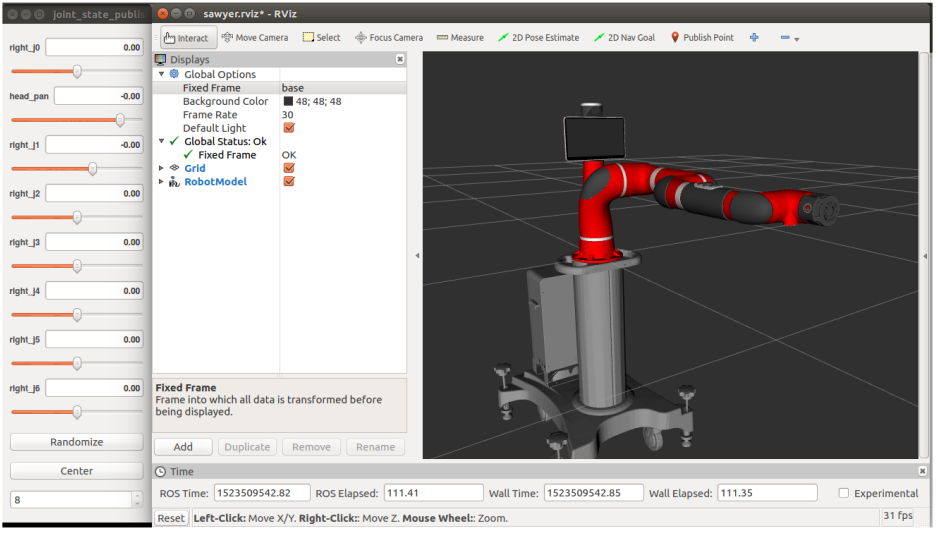
\includegraphics[width=1.0\textwidth]{robot.png}
   \caption{Sawyer robot in RViz.}
   \label{fig:sawyer}
\end{figure}

With the sliders you can move each robot joint. Try moving the joints! The model that RViz shows is purely kinematic; that is, the weights of the rigid bodies, or the external forces are not taken into account. Collisions are not taken into account either (you might see the robot colliding with itself without any physical consequence). To close RViz, type
Ctrl+c in the terminal where roslaunch was executed.

The URDF model of other manipulators, mobile robots, humanoid robots, aerial robots, among other types of robots, can be downloaded from https://wiki.ros.org/Robots. For any robot, if the URDF model is in xacro format, the launch file needed to show it in RViz is similar to the one developed for Sawyer.

\textbf{Frames}. Each rigid body that composes the robot has a frame that is attached to it.To see these frames, add one element of type TF : Add → TF. In the left panel, in the TF part, it is suggested to disable the following options: Show Names, and Show Arrows. Only Show Axes must be checked. By convention, the order of the axis is given in RGB format: red represents x, green represents y, and blue represents axis z. Note that when you move the sliders, some frames also move.

\section{Questions}
\begin{itemize}
\item How many degrees of freedom does Sawyer have?
\item Based on the robot model shown in RViz, what are the joint limits of Sawyer? That is, what are the maximum and minimum values that each joint can take?
\item Moving the sliders, find a feasible configuration (without collisions) such that the orientation of the end effector with respect to the base of the robot is given by:
\begin{equation}
R = [-1,0,0; 0,0,1; 0,1,0]
\end{equation}
\item First you might want to only show the frames for the base and the right hand. Write the joint configuration (angles for every joint) you found, and add a screenshot showing the achieved task.
\item Determine the names of the joints extracting information from the message that is set from the sliders to the visualizer. Type rostopic echo /joint states and write the joint names, which can be found as ''name''. Also, add a screenshot of the terminal output showing these names.
\end{itemize}
\end{document}

\end{document}